\documentclass{beamer}
\usepackage{default}
\usepackage{amsmath}
\usepackage{graphicx}
\usepackage{adjustbox}  % Allows for fitting tables into slide
\usepackage{hyperref}
\usepackage{threeparttable}
\usepackage{caption}
%\usepackage{subcaption}
\usepackage{natbib}
\usepackage{adjustbox}
\usepackage{subcaption}




%\usetheme{AnnArbor}
%\usetheme{Antibes}
%\usetheme{Bergen}
%\usetheme{Berkeley}
%\usetheme{Berlin}
%\usetheme{Boadilla}
%\usetheme{boxes}
\usetheme{CambridgeUS}
%\usetheme{Copenhagen}
%\usetheme{Darmstadt}
%\usetheme{default}
%\usetheme{Frankfurt}
%\usetheme{Goettingen}
%\usetheme{Hannover}
%\usetheme{Ilmenau}
%\usetheme{JuanLesPins}
%\usetheme{Luebeck}
%\usetheme{Madrid}
%\usetheme{Malmoe}
%\usetheme{Marburg}
%\usetheme{Montpellier}
%\usetheme{PaloAlto}
%\usetheme{Pittsburgh}
%\usetheme{Rochester}
%\usetheme{Singapore}
%\usetheme{Szeged}
%\usetheme{Warsaw}

% colortheme to choose one 

%\usecolortheme{beaver}
%\usecolortheme{crane}
%\usecolortheme{default}
\usecolortheme{dolphin}
%\usecolortheme{seagull}
%\usecolortheme{seahorse}
%\usecolortheme{whale}


% fond theme to choose one 
%\usefonttheme{structuresmallcapsserif}
%\usefonttheme{structureitalicserif}
%\usefonttheme{structurebold}
\usefonttheme{serif}
%\usefonttheme{professionalfonts}
%\usefonttheme{default}

\title{Perceived Income Risks}


% A subtitle is optional and this may be deleted

\author{Tao Wang \\ Johns Hopkins University}
% - Give the names in the same order as the appear in the paper.
% - Use the \inst{?} command only if the authors have different
%   affiliation.

\date{\today}
% - Either use conference name or its abbreviation.
% - Not really informative to the audience, more for people (including
%   yourself) who are reading the slides online

% This is only inserted into the PDF information catalog. Can be left
% out. 

% If you have a file called "university-logo-filename.xxx", where xxx
% is a graphic format that can be processed by latex or pdflatex,
% resp., then you can add a logo as follows:

% \pgfdeclareimage[height=0.5cm]{university-logo}{university-logo-filename}
% \logo{\pgfuseimage{university-logo}}

% Delete this, if you do not want the table of contents to pop up at
% the beginning of each subsection:
\AtBeginSubsection[]
{
	\begin{frame}<beamer>{Outline}
	\tableofcontents[currentsection]
\end{frame}
}

\begin{document}
	

\begin{frame}
	\titlepage
\end{frame}
\begin{frame}{Outline}
	\tableofcontents
	% You might wish to add the option [pausesections]
\end{frame}


\section{Motivation}

\begin{frame}{Motivation}
	\begin{itemize}
		\item ddddddddd
	\end{itemize}
\end{frame}


\begin{frame}{This paper's agenda}
	\begin{enumerate}
		\item dddd
	\end{enumerate}
\end{frame}


\begin{frame}{Literature}
\begin{itemize}
	\item ddddd
	\begin{itemize}
		\item dddd
	\end{itemize}
\end{itemize}
\end{frame}

\section{Stylized facts}


\begin{frame}{Data}
	\begin{table}
		\centering
		\caption{Survey of Consumer Expectations}
		\label{SCE_data_sum}
		\adjustbox{max height=0.5\textheight, max width=\textwidth}{ 
			\begin{tabular}{lll}
				\hline 
				Time period                                    & 2013M6-2018M6            \\
				Frequency                                      & monthly                                 \\
				Sample size                                    & 1,300                                  \\
				Density variable                    &  \textcolor{blue}{1-yr-ahead earning growth   (same position/hours) }           \\
				Pannel structure                               & stay up to 12 months      \\
				Demographics                     & educ, income, age        \\
				\hline 
			\end{tabular}
		}
	\end{table}
	\begin{itemize}
		\item density estimation following (\cite{engelberg_comparing_2009})
		\item exclude top and bottom 5\% values for forecast errors and uncertainty
	\end{itemize}
\end{frame}


\begin{frame}{Definitions}
	\begin{itemize}
		\item Moments to look at 
		\begin{itemize}
			\item expected growth, $\overline \Delta_i (y_i)$
			\item variance: $\overline {var}_i(\Delta y_i)$
			\item skewness: $\overline {skew}_i(\Delta y_i)$
		\end{itemize}
		\item Nominal can be converted into real using forecast uncertainty of inflation 
		\begin{itemize}
			\item $\overline{var}_i(\Delta y^r) =\overline {var}_i(\Delta y^n) +  \overline {var}_i(\pi)$
		\end{itemize}
		\item Also, can be adjusted with perceived unemployment risk. So the perceived risk of same job/hour is just a lower bound for income risk. 
	\end{itemize}
\end{frame}

\subsection{Cross-sectional pattern of subjective income risks}

\begin{frame}{Cross-sectional distribution of expected income growth}
	\begin{figure}
		\centering
		\label{incexp_hist}
		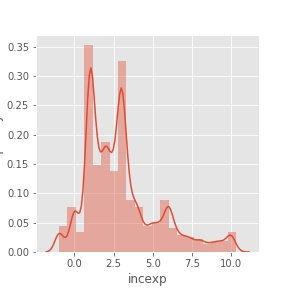
\includegraphics[width=0.4\textwidth]{figures/hist_incexp}
		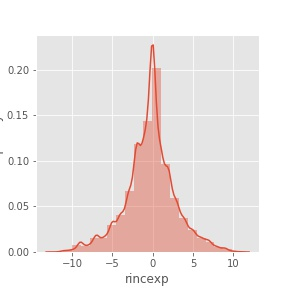
\includegraphics[width=0.4\textwidth]{figures/hist_rincexp} 
	\end{figure}
	\begin{itemize}
		\item Nominal rigity can be seen from the expected norminal earning growth, while real expected growth become symmetric 
	\end{itemize}
\end{frame}

\begin{frame}{Cross-sectional distribution of income dispersion}
	\begin{figure}
		\centering
		\label{incvar_hist}
		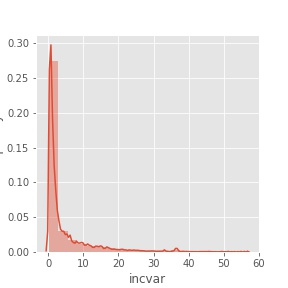
\includegraphics[width=0.4\textwidth]{figures/hist_incvar}
		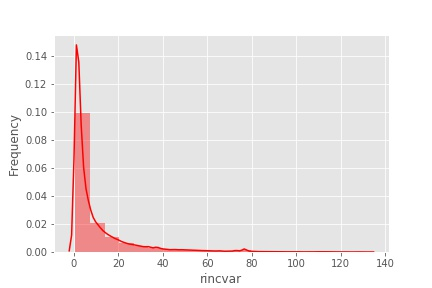
\includegraphics[width=0.4\textwidth]{figures/hist_rincvar}
	\end{figure}
	\begin{itemize}
		\item average perceived income risks:  $3\%$ standard deviation for nominal and $4\%$ standard deviation for real income
		\item just a lower bound: before adjustment of unemployment risk 
	\end{itemize}
\end{frame}

\begin{frame}{Cross-sectional distribution of tail risks}
	\begin{figure}
		\centering
		\label{incvar_skew}
		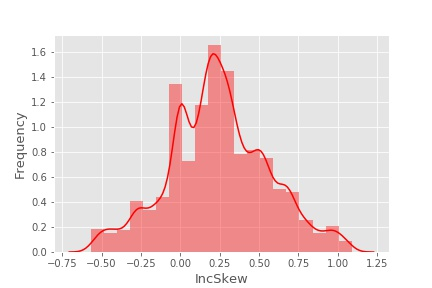
\includegraphics[width=0.4\textwidth]{figures/histIncSkew}
	\end{figure}
	\begin{itemize}
		\item sizable dispersion in skewness, i.e. about half of the people have non-zero skewness in perceived inome distribution. 
	\end{itemize}
\end{frame}


\begin{frame}{Perceived income risks by household income}
	\begin{figure}
		\centering
		\label{boxplot_hhinc}
		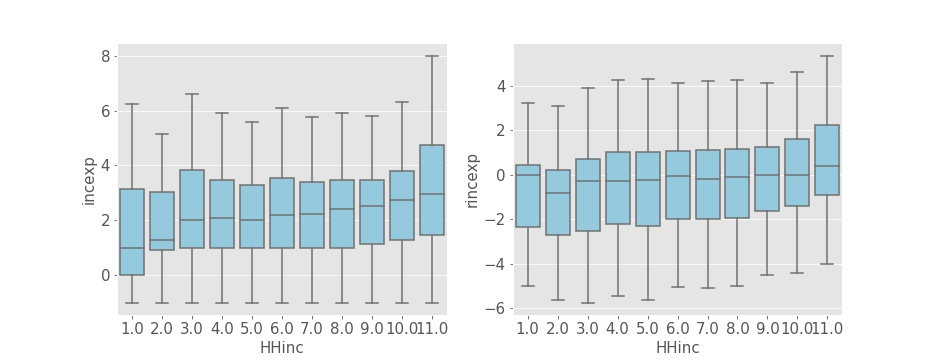
\includegraphics[width=0.8\textwidth]{figures/boxplot_exp_HHinc} \\
		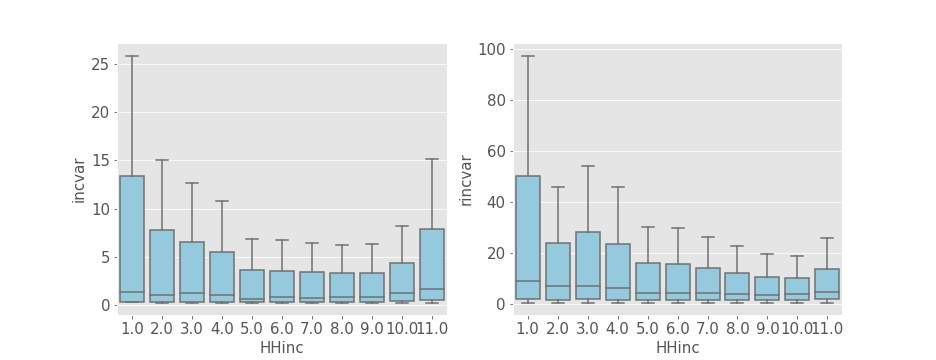
\includegraphics[width=0.8\textwidth]{figures/boxplot_var_HHinc}
	\end{figure}
	\begin{itemize}
		\item 
	\end{itemize}
\end{frame}


\begin{frame}{Perceived income risks by age}
	\begin{figure}
		\centering
		\label{boxplot_age_gr}
		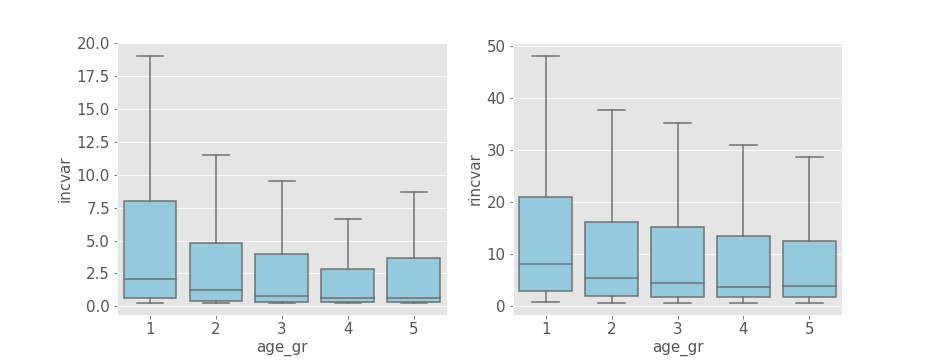
\includegraphics[width=0.8\textwidth]{figures/boxplot_exp_age_gr} \\
		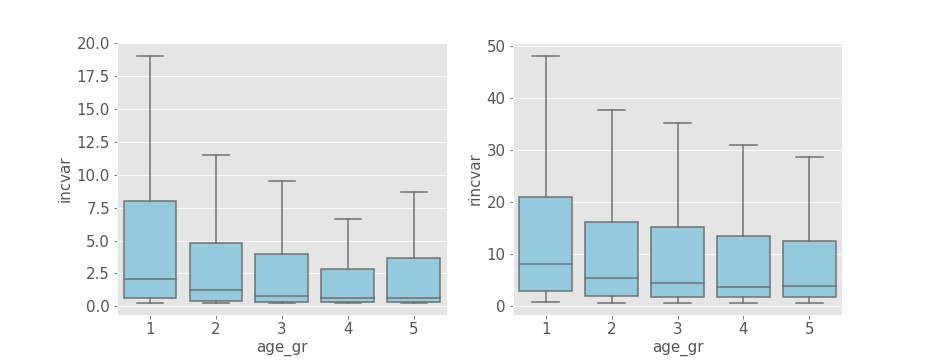
\includegraphics[width=0.8\textwidth]{figures/boxplot_var_age_gr}
	\end{figure}
	\begin{itemize}
		\item 
	\end{itemize}
\end{frame}



\begin{frame}{Perceived income risks by generation}
	\begin{figure}
		\centering
		\label{boxplot_byear_gr}
		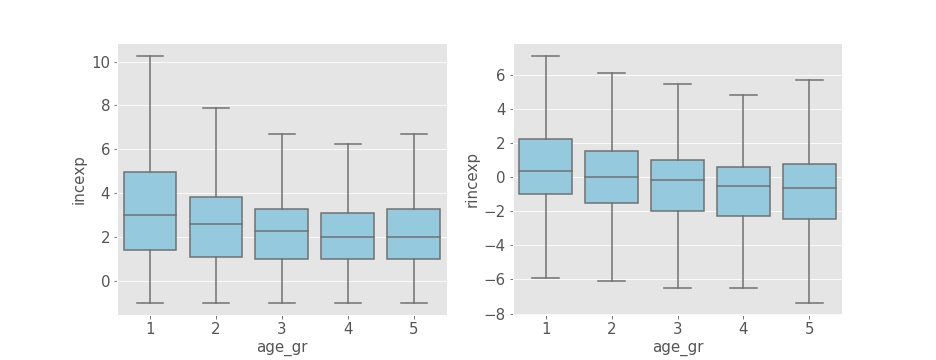
\includegraphics[width=0.8\textwidth]{figures/boxplot_exp_byear_gr} \\
		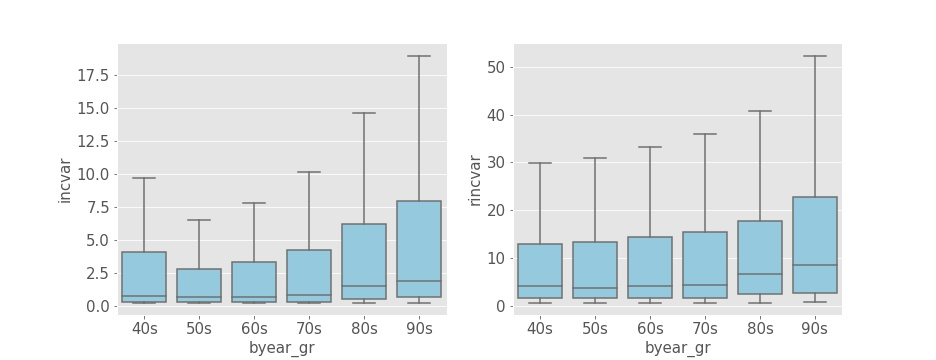
\includegraphics[width=0.8\textwidth]{figures/boxplot_var_byear_gr}
	\end{figure}
	\begin{itemize}
		\item 
	\end{itemize}
\end{frame}


\begin{frame}{Covariants of expected income growth}
	\begin{table}
		\centering
		\caption{Expected income growth and individual characteristics}
		\label{micro_reg_exp}
		\adjustbox{max height=0.5\textheight, max width=\textwidth}{ 
			\begin{tabular}{ccccccccc}
				\hline 
				{} &  incexp I & incexp II & incexp III & incexp IIII & rincexp I & rincexp II & rincexp III & rincexp IIII \\
				\hline 
				HHinc\_gr=low inc &           &           &      -0.03 &             &           &            &    -0.39*** &              \\
				&           &           &     (0.02) &             &           &            &      (0.03) &              \\
				educ\_gr=low educ &           &           &            &    -0.25*** &           &            &             &     -0.63*** \\
				&           &           &            &      (0.02) &           &            &             &       (0.03) \\
				gender=male      &           &           &            &    -0.32*** &           &            &             &     -0.78*** \\
				&           &           &            &      (0.02) &           &            &             &       (0.03) \\
				parttime=yes     &  -0.47*** &  -0.36*** &   -0.35*** &             &  -0.63*** &   -0.53*** &    -0.44*** &              \\
				&    (0.03) &    (0.03) &     (0.03) &             &    (0.04) &     (0.04) &      (0.04) &              \\
				selfemp=yes      &   0.86*** &  -0.00*** &    0.00*** &             &   0.84*** &   -0.00*** &    -0.00*** &              \\
				&    (0.03) &    (0.00) &     (0.00) &             &    (0.05) &     (0.00) &      (0.00) &              \\
				Stkprob          &           &   0.01*** &    0.01*** &             &           &    0.02*** &     0.02*** &              \\
				&           &    (0.00) &     (0.00) &             &           &     (0.00) &      (0.00) &              \\
				UEprobInd        &           &  -0.01*** &   -0.01*** &             &           &   -0.02*** &    -0.02*** &              \\
				&           &    (0.00) &     (0.00) &             &           &     (0.00) &      (0.00) &              \\
				Intercept        &   2.82*** &   2.57*** &    2.58*** &     3.05*** &  -0.29*** &   -0.92*** &    -0.80*** &      0.20*** \\
				&    (0.01) &    (0.02) &     (0.02) &      (0.02) &    (0.02) &     (0.03) &      (0.03) &       (0.02) \\
				\hline 
				N                &     54275 &     48606 &      48606 &       47712 &     49702 &      44446 &       44446 &        43694 \\
				R2               &      0.01 &      0.02 &       0.02 &        0.01 &      0.01 &       0.04 &        0.04 &         0.02 \\
				
				\hline 
			\end{tabular}
		}
	\end{table}
\end{frame}

\begin{frame}{Covariants of perceived income risks}
	\begin{table}
		\centering
		\caption{Perceived income risks and individual characteristics}
		\label{micro_reg}
		\adjustbox{max height=0.5\textheight, max width=\textwidth}{ 

\begin{tabular}{ccccccccc}
	\hline 
	{} &  incexp I & incexp II & incexp III & incexp IIII & rincexp I & rincexp II & rincexp III & rincexp IIII \\
	\hline 
	HHinc\_gr=low inc &           &           &      -0.03 &             &           &            &    -0.36*** &              \\
	&           &           &     (0.02) &             &           &            &      (0.03) &              \\
	educ\_gr=low educ &           &           &            &    -0.25*** &           &            &             &     -0.63*** \\
	&           &           &            &      (0.02) &           &            &             &       (0.03) \\
	gender=male      &           &           &            &    -0.32*** &           &            &             &     -0.78*** \\
	&           &           &            &      (0.02) &           &            &             &       (0.03) \\
	parttime=yes     &  -0.47*** &  -0.36*** &   -0.36*** &             &  -0.63*** &   -0.53*** &    -0.45*** &              \\
	&    (0.03) &    (0.03) &     (0.03) &             &    (0.04) &     (0.04) &      (0.04) &              \\
	selfemp=yes      &   0.86*** &   0.00*** &    0.00*** &             &   0.84*** &   -0.00*** &    -0.00*** &              \\
	&    (0.03) &    (0.00) &     (0.00) &             &    (0.05) &     (0.00) &      (0.00) &              \\
	Stkprob          &           &   0.01*** &    0.01*** &             &           &    0.02*** &     0.02*** &              \\
	&           &    (0.00) &     (0.00) &             &           &     (0.00) &      (0.00) &              \\
	UEprobAgg        &           &  -0.00*** &   -0.00*** &             &           &   -0.01*** &    -0.01*** &              \\
	&           &    (0.00) &     (0.00) &             &           &     (0.00) &      (0.00) &              \\
	UEprobInd        &           &  -0.01*** &   -0.01*** &             &           &   -0.01*** &    -0.01*** &              \\
	&           &    (0.00) &     (0.00) &             &           &     (0.00) &      (0.00) &              \\
	Intercept        &   2.82*** &   2.63*** &    2.64*** &     3.05*** &  -0.29*** &   -0.52*** &    -0.41*** &      0.20*** \\
	&    (0.01) &    (0.03) &     (0.03) &      (0.02) &    (0.02) &     (0.04) &      (0.04) &       (0.02) \\           
	\hline 
	N                &     54275 &     48579 &      48579 &       47712 &     49702 &      44424 &       44424 &        43694 \\
	R2               &      0.01 &      0.02 &       0.02 &        0.01 &      0.01 &       0.05 &        0.05 &         0.02 \\
	\hline 
\end{tabular}	
}
	\end{table}
\end{frame}


\subsection{Perceived risks and economic decisions}


\begin{frame}{Perveived Income Risks and Household Spending}
	\begin{table}
		\centering
		\caption{Perceived income risks and household spending}
		\label{spending_reg}
		\adjustbox{max height=0.5\textheight, max width=\textwidth}{ 
	
	\begin{tabular}{ccccccll}
		\hline 
		{} & spending I & spending II & spending III & spending IIII & spending IIIII & spending IIIIII & spending IIIIIII \\
		\hline 
		incexp    &    0.39*** &             &              &               &                &                 &                  \\
		&     (0.08) &             &              &               &                &                 &                  \\
		
		rincexp   &            &      -0.04* &              &               &                &                 &                  \\
		&            &      (0.02) &              &               &                &                 &                  \\
		incvar    &            &             &      0.07*** &               &                &                 &                  \\
		&            &             &       (0.02) &               &                &                 &                  \\
		
		rincvar   &            &             &              &       0.07*** &                &                 &                  \\
		&            &             &              &        (0.01) &                &                 &                  \\
		
		UEprobAgg &            &             &              &               &                &         0.04*** &                  \\
		&            &             &              &               &                &          (0.01) &                  \\
		UEprobInd &            &             &              &               &          -0.01 &                 &                  \\
		&            &             &              &               &         (0.01) &                 &                  \\
		
		incskew   &            &             &              &               &                &                 &             0.21 \\
		&            &             &              &               &                &                 &           (0.43) \\
		\hline 
		N         &      55673 &       50997 &        55465 &         52099 &          54315 &           85468 &            55029 \\
		R2        &       0.00 &        0.00 &         0.00 &          0.00 &           0.00 &            0.00 &             0.00 \\
		\hline 
	\end{tabular}
		}
	\end{table}
\end{frame}


\subsection{Correlation with stock market returns}

\begin{frame}{Expected income growth and stock market performance}
		\begin{figure}
		\centering
		\label{ts_mean}
		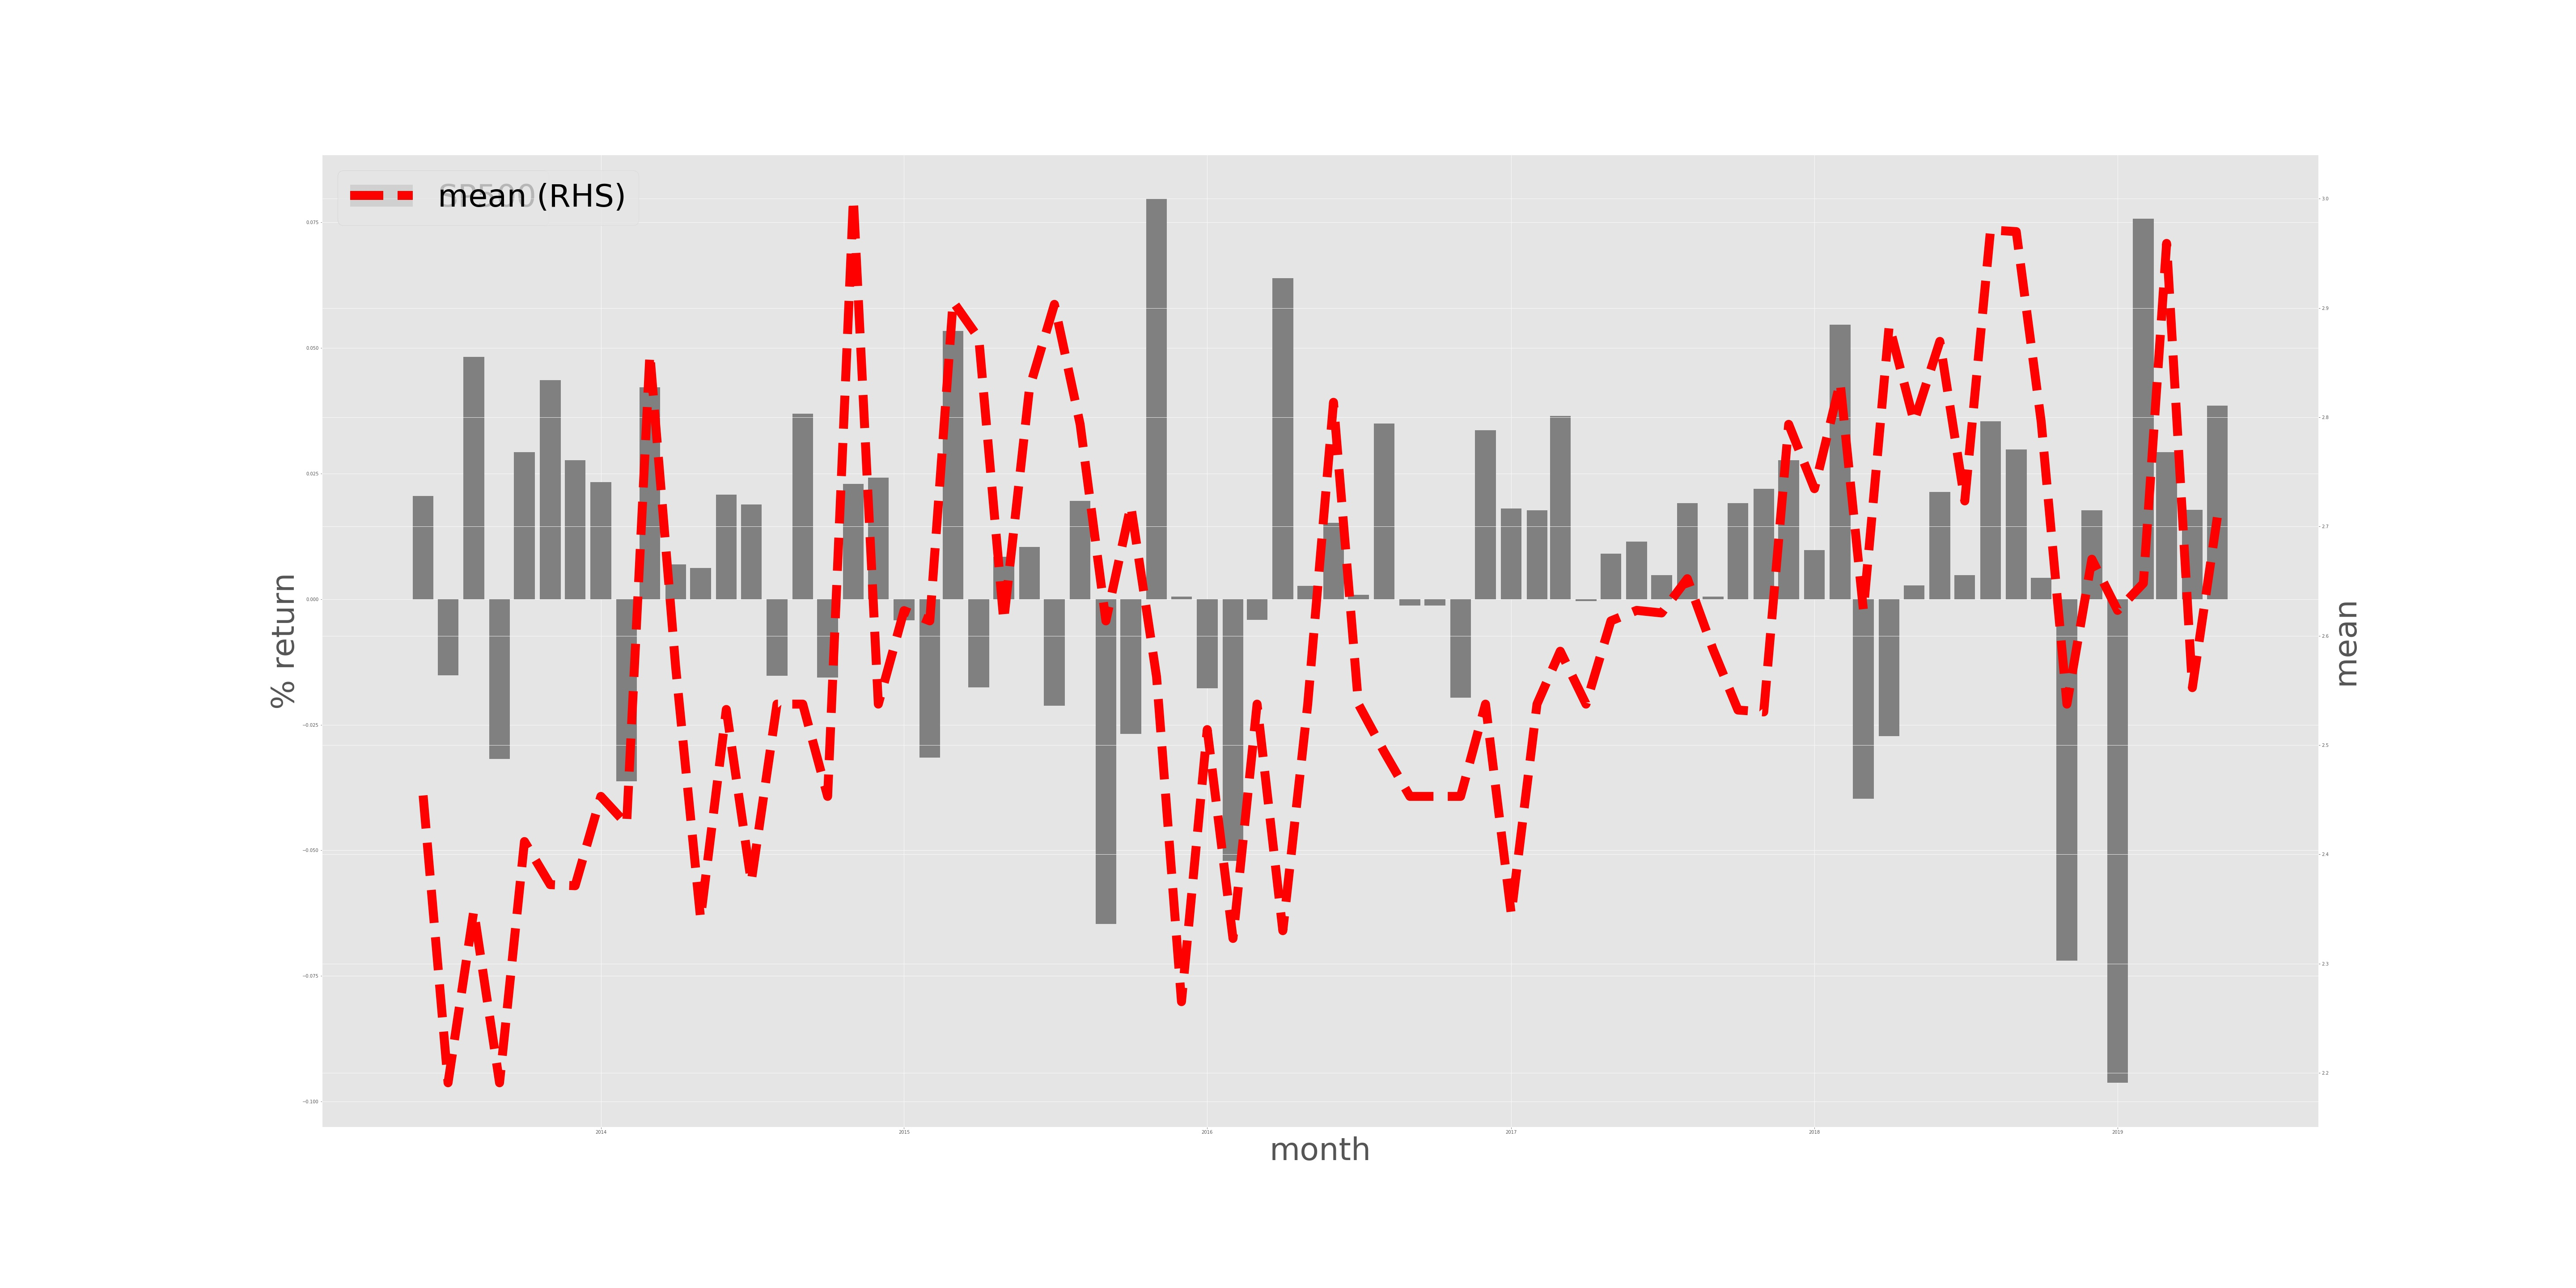
\includegraphics[width=\textwidth]{figures/tsMedmean.jpg}
	\end{figure}
	\begin{itemize}
		\item 
	\end{itemize}
\end{frame}


\begin{frame}{Dispersion risks and stock market performance}
	\begin{figure}
		\centering
		\label{ts_var}
		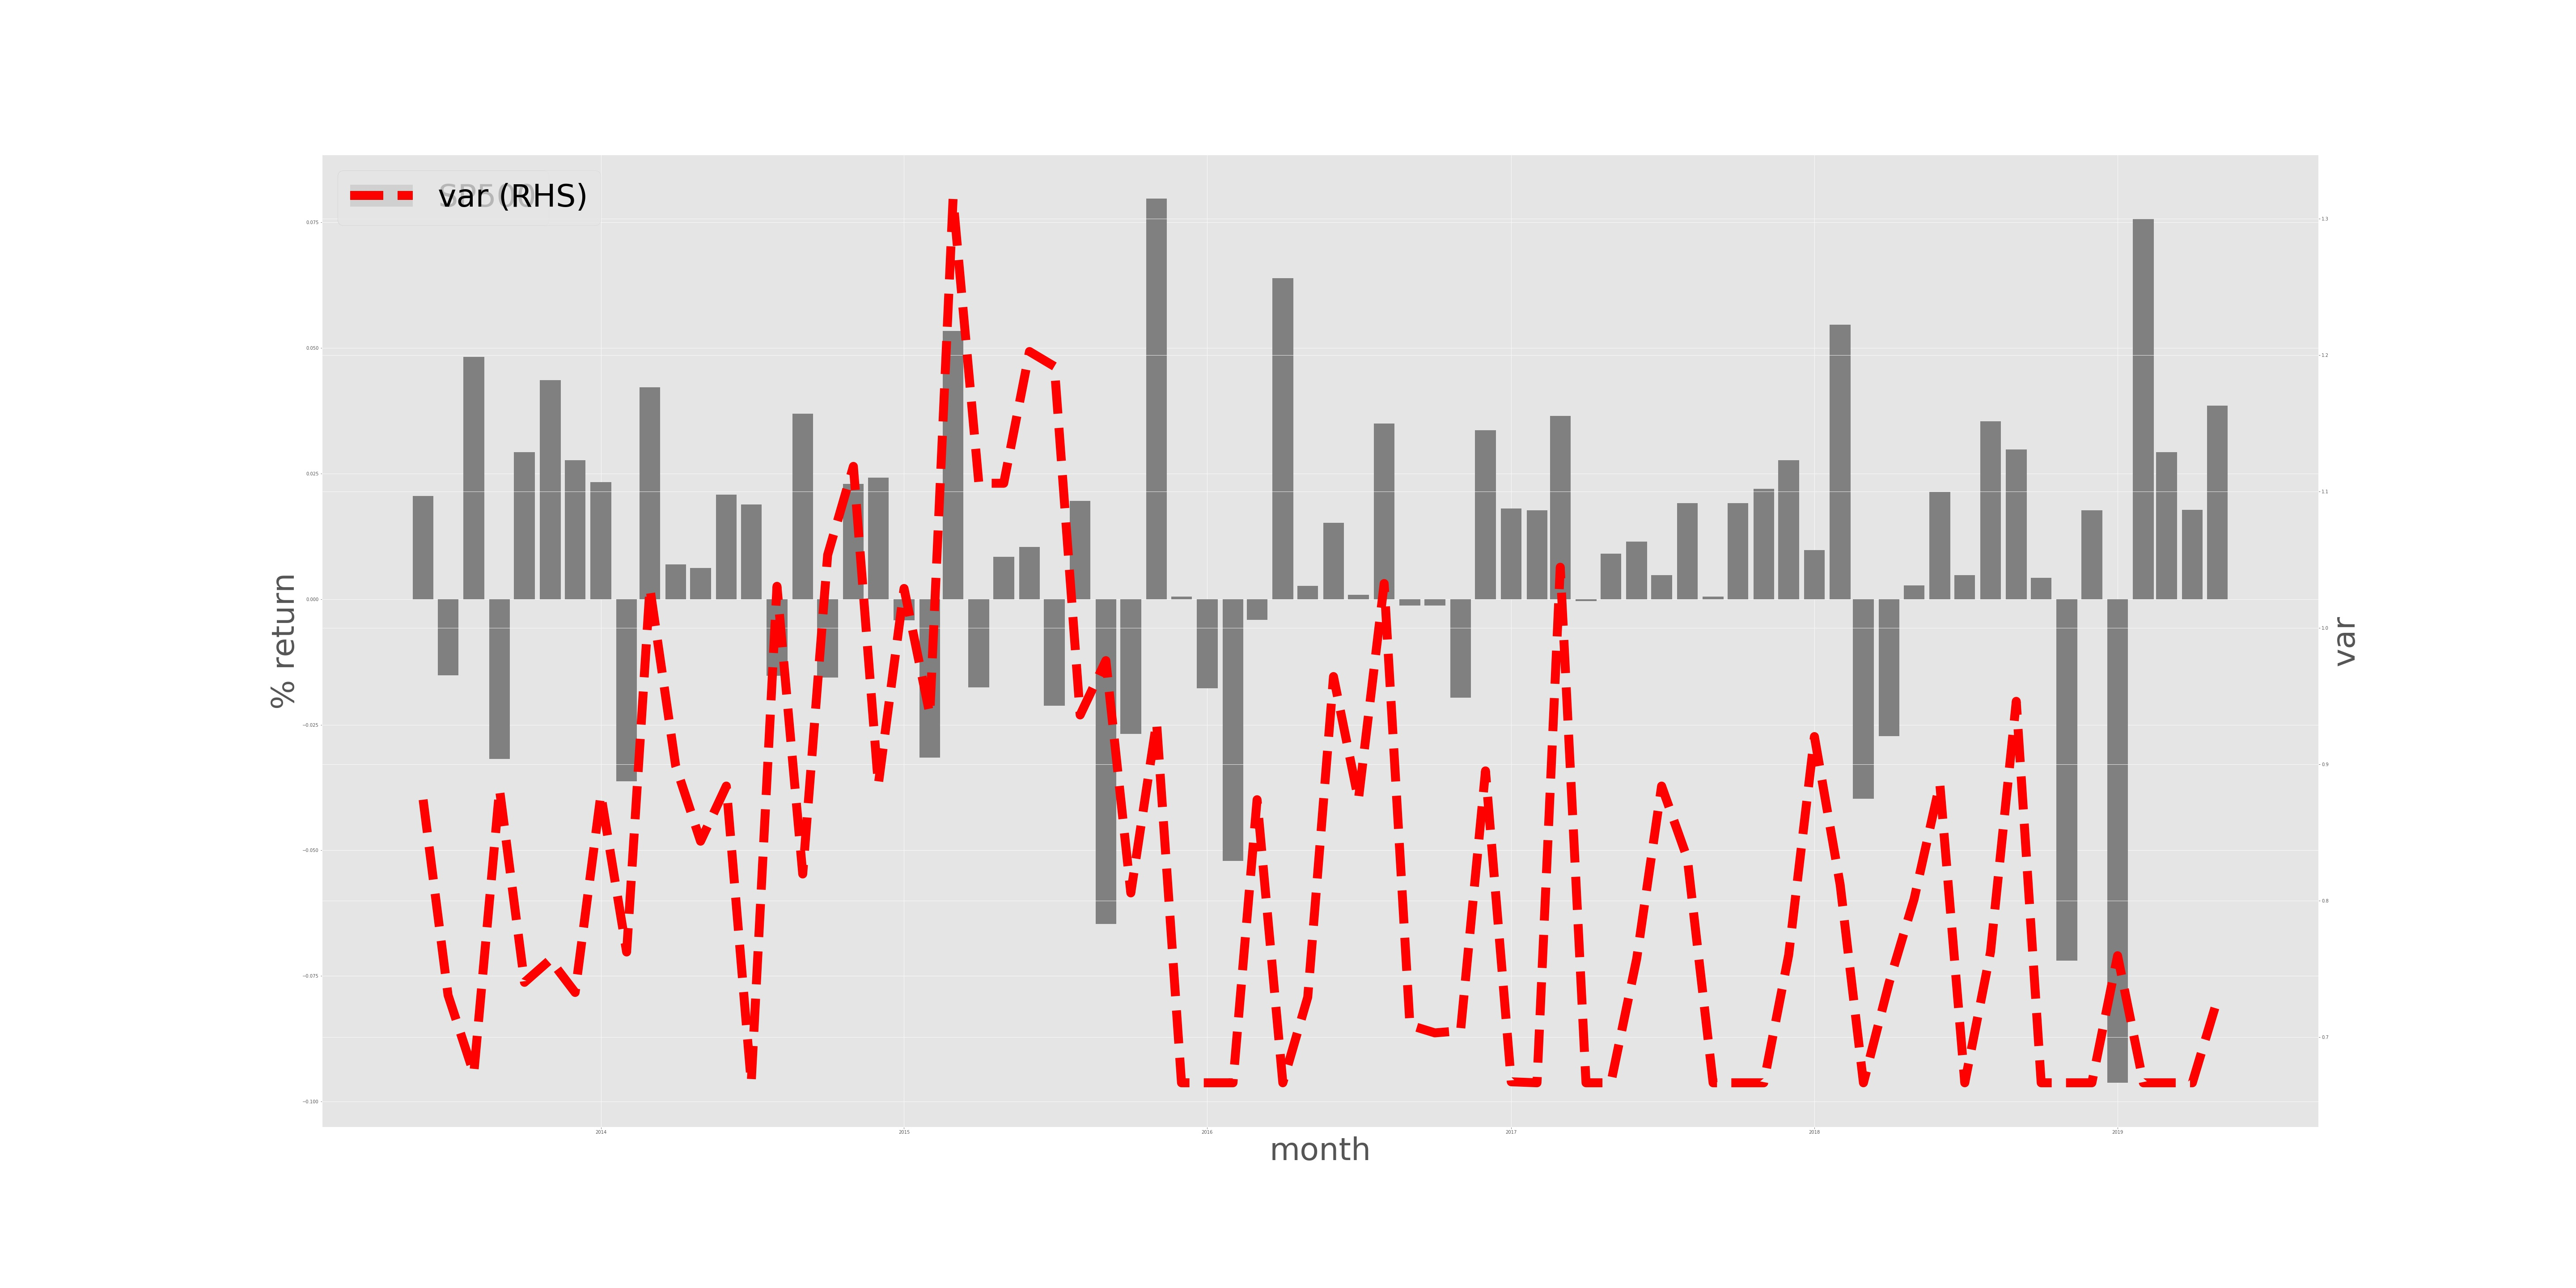
\includegraphics[width=\textwidth]{figures/tsMedvar.jpg}
	\end{figure}
	\begin{itemize}
		\item 
	\end{itemize}
\end{frame}



\begin{frame}{Tail risks and stock market performance}
	\begin{figure}
		\centering
		\label{ts_skew}
		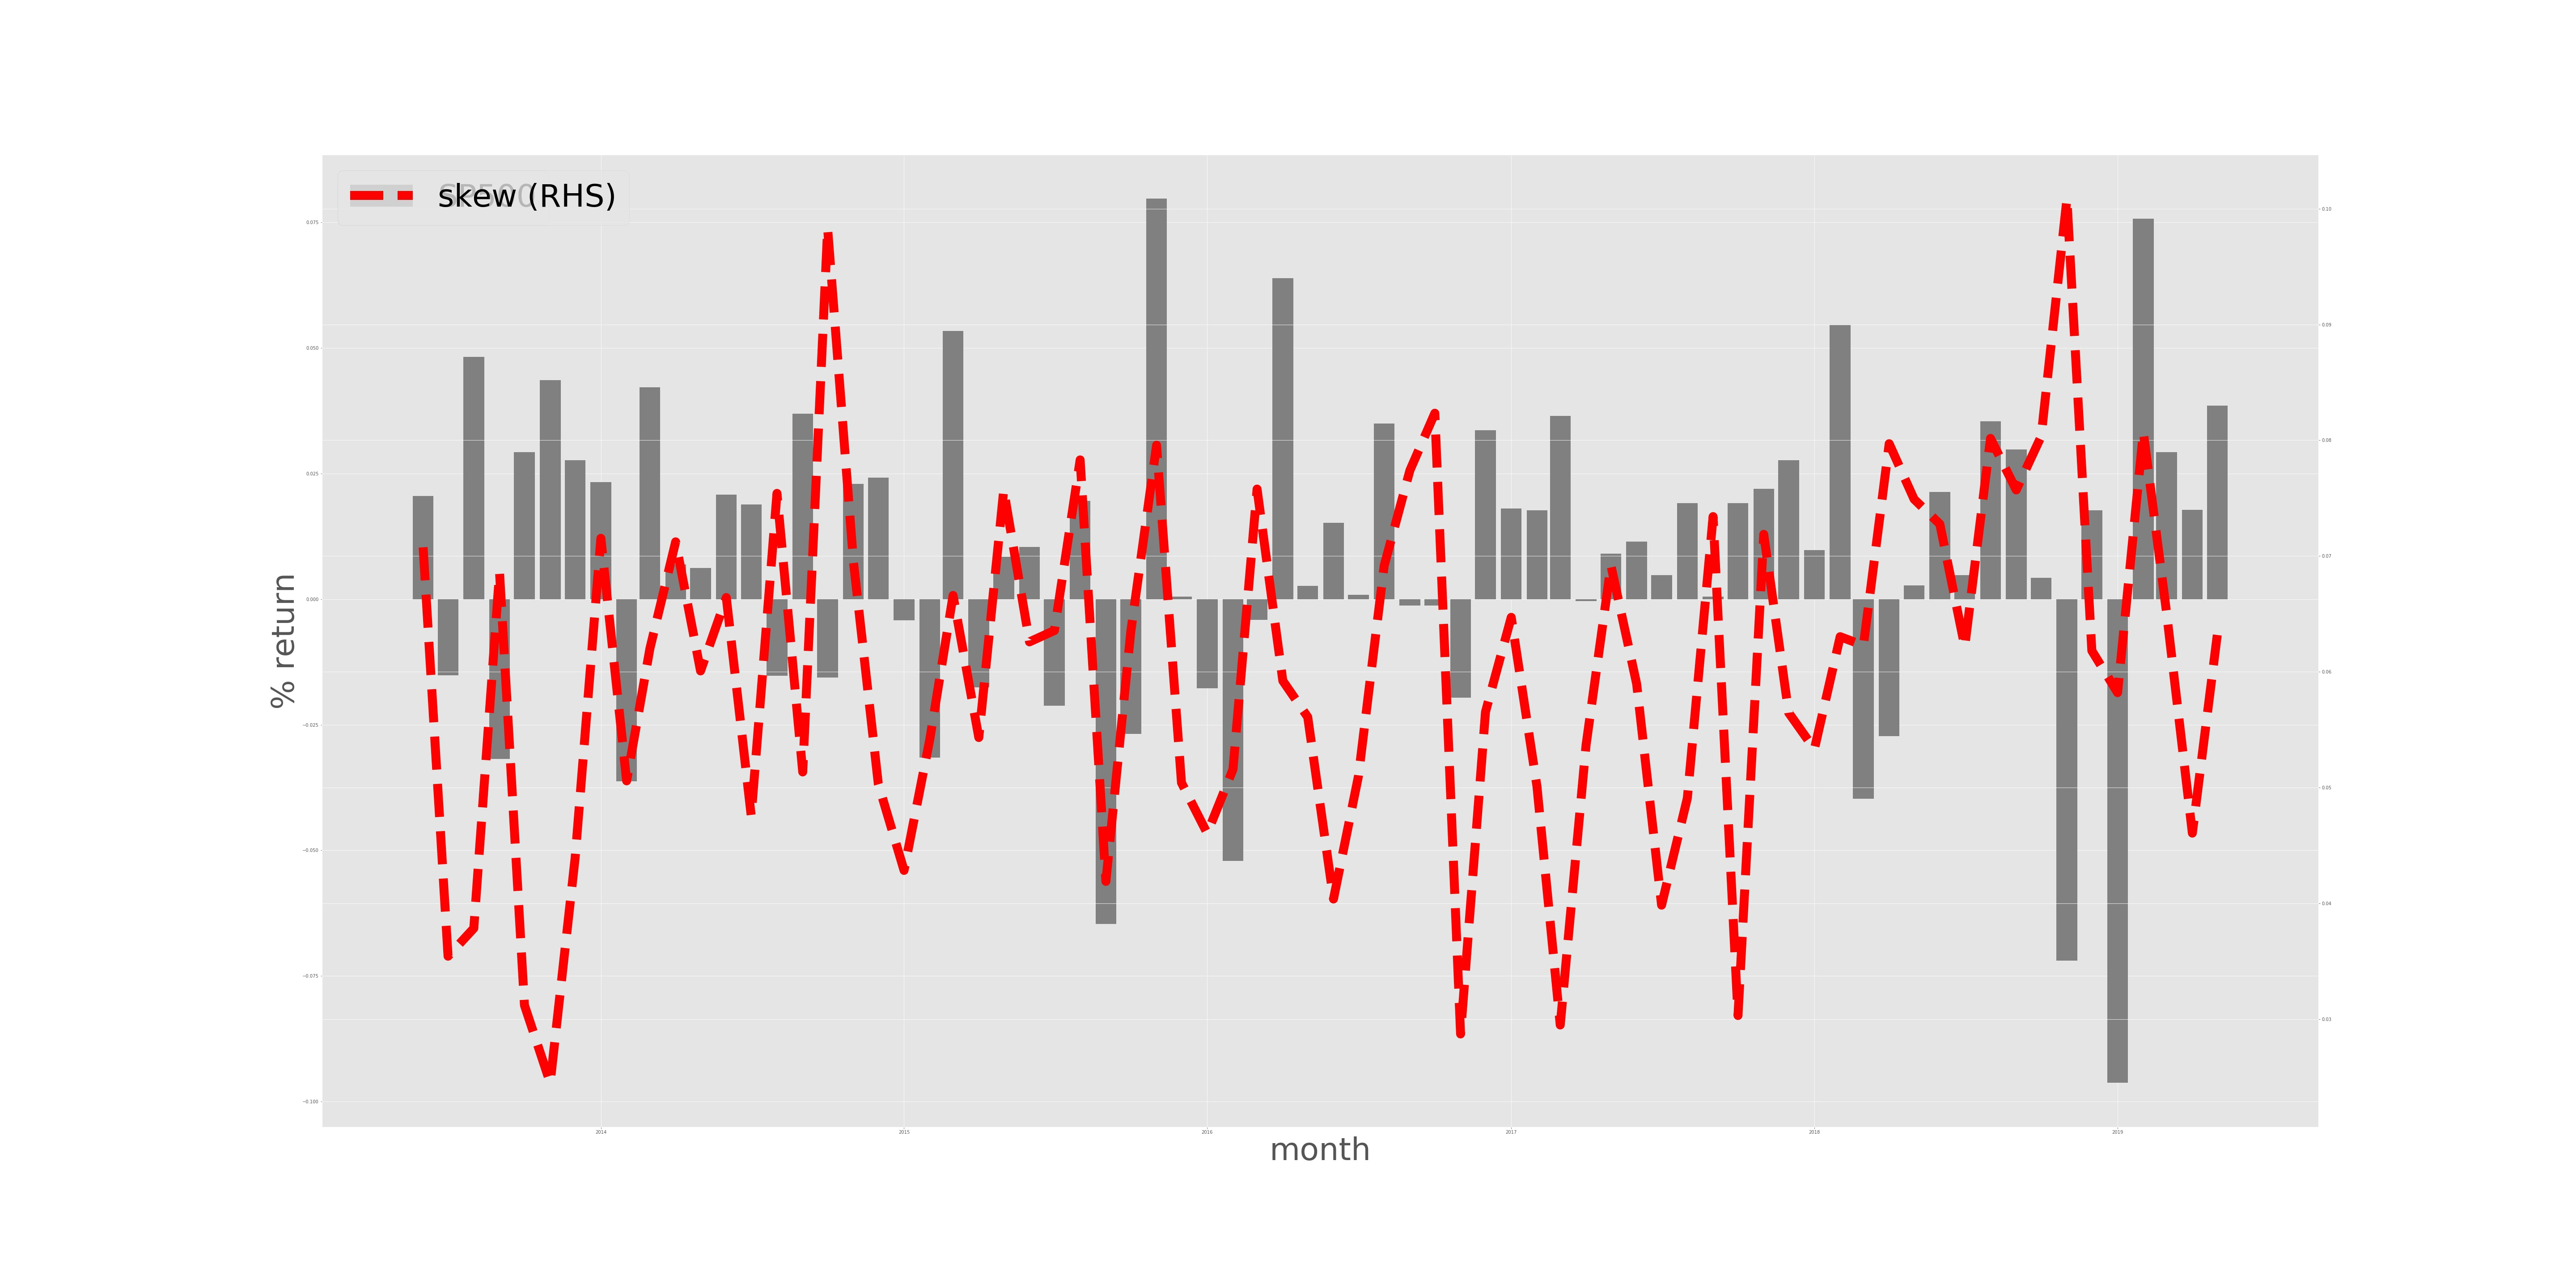
\includegraphics[width=\textwidth]{figures/tsEstMeanskew.jpg}
	\end{figure}
	\begin{itemize}
		\item 
	\end{itemize}
\end{frame}


\section{Model (work in progress)}

\begin{frame}{Model ingredients}
	
	\begin{enumerate}
		\item imperfect understanding of the income process, a deviation from rational expectation benchmark. 
		\begin{itemize}
			\item experience-based learning capturing the cross-generatio and age-dependence income perceptions
		\end{itemize}
		\item finite-period life cycle with a constant probability of death 
		\item uninsured idiosyncratic risks and aggregate risks, workhorse assumption of the HANK literature
		\item single asset, i.e. no distinction between liquid and iliquid assets 
	\end{enumerate}
\end{frame}

\begin{frame}{Intuitions behind the model mechanisms}
	\begin{itemize}
		\item imperfect understanding $ \quad \rightarrow$ heterogeneous perception of risks $ \quad \plus$ uninsurance of risks $ \quad \rightarrow$ difference in precautionary motives and MPCs across populations $ \quad \rightarrow$ potential amplification of aggregate MPC. 
	\end{itemize}
\end{frame}

%%%%%%%%%%%%%%%%%%%


\begin{frame}{Some Figures}
	\begin{figure}[ht]
		\label{figurelabel}
		\begin{subfigure}[b]{0.2\textwidth}
			\centering
			\caption{FE}
			\includegraphics[width=\textwidth, height = 0.8\textheight]{figuresDraft/spf_se_est_diag0.png}
		\end{subfigure}
		\hfill
		\begin{subfigure}[b]{0.2\textwidth}
			\caption{Disg}
			\includegraphics[width=\textwidth, height = 0.8\textheight]{figuresDraft/spf_se_est_diag1.png}
		\end{subfigure}
		\hfill
		\begin{subfigure}[b]{0.2\textwidth}
			\caption{FE/Disg}
			\includegraphics[width=\textwidth, height = 0.8\textheight]{figuresDraft/spf_se_est_diag2.png}
		\end{subfigure}
	\end{figure}
\end{frame}


%%%%%%%%%%%%%%%%%%%%%%%%%%%%%%%%%


\section{Conclusion}

\begin{frame}{Conclusion}
	\begin{itemize}
		\item ddddd
	\end{itemize}	
\end{frame}

\section*{Appendix}

\begin{frame}{Density estimation and robustness of my results}
	\begin{itemize}
		\item ddd
	\end{itemize}
\end{frame}


\bibliographystyle{apalike}
\bibliography{PerceivedIncomeRisk}


\end{document}
